\chapter{Additional Results}
\label{app:additional-results}

This appendix gives additional simulation results and supporting checks
for Chapter~\ref{chap:results}, followed by Holm's multiple-testing adjustment
for the online-shopping application. Each simulation setting uses 20,000
sampled table pairs and a two-sided 5\% test. Rejection rates divide valid
rejections by all repetitions; brackets around rejection rates and error
bands give pointwise Wilson 95\% intervals. All test results and diagnostics outside the
equal-MI study are finite and valid.

\section{Additional equal-MI comparisons}

Figure~\ref{fig:focused-null-remaining} supplies the four size--margin
curves not displayed in the main null figures: uniform and same-skew
\(2\times2\) and \(8\times8\) populations. Both population MI values
are 0.02 nats, with margins from Table~\ref{tab:margin-profiles}.
The lower strips show validity.

\begin{figure}[H]
\centering
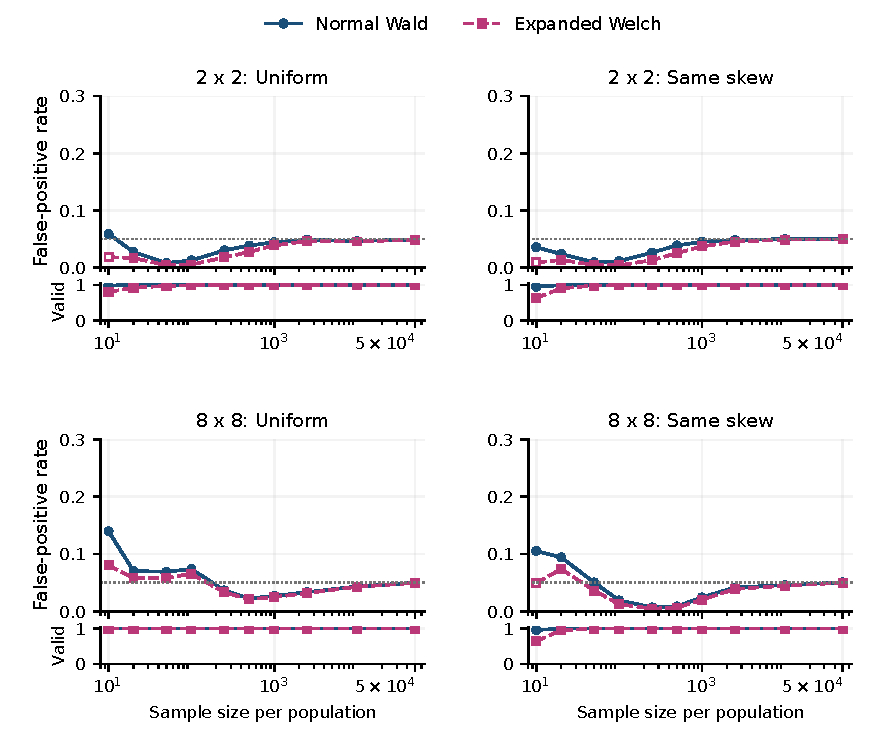
\includegraphics{focused_null_remaining.pdf}
\caption{Additional equal-MI comparisons under uniform and same-skew margins.}
\label{fig:focused-null-remaining}
\end{figure}

The \(2\times2\) comparisons give low false-positive rates at
intermediate sample sizes. At \(8\times8\) and \(n=100\), rejection
is excessive under uniform margins but conservative under same skew.
By \(n=50{,}000\), all four comparisons have rates between 0.0490
and 0.0503 and full validity.

\section{Supporting estimation diagnostics}

In the diagnostic and supporting-check tables below, Bias is the mean
error in the corrected MI difference; observed SD is its standard
deviation across samples, both in nats. Est./obs. divides the mean squared
standard error by the observed sampling variance; Pop./obs. uses the
population first-order variance in the numerator. DF is the median
combined degrees of freedom, with the 5th--95th percentile range where
shown. W/E denotes Normal Wald and Expanded Welch. The variance-estimate
ratios in Table~\ref{tab:variance-stability} are defined separately below.

Table~\ref{tab:association-diagnostics} gives the diagnostics behind
the population-MI comparison in Figure~\ref{fig:focused-association}.
Here the population first-order variance is \(V(P)/n+V(Q)/n\).

\begin{table}[H]
\centering
\small
\caption{Diagnostics for \(4\times4\) different-skew populations with equal MI.}
\label{tab:association-diagnostics}
\begin{tabular}{@{}rrrrrr@{}}\toprule
\(n\) & MI & Bias & DF median [5th, 95th] & Est./obs. & Pop./obs.\\\midrule
100 & 0.0001 & 0.00751 & 4.23 [2.25, 8.77] & 1.919 & 0.007\\
100 & 0.0003 & 0.00724 & 4.33 [2.27, 9.11] & 1.850 & 0.019\\
100 & 0.001 & 0.00666 & 4.53 [2.32, 9.62] & 1.851 & 0.062\\
100 & 0.003 & 0.00606 & 4.98 [2.45, 10.63] & 1.760 & 0.166\\
100 & 0.01 & 0.00567 & 6.35 [2.92, 13.61] & 1.611 & 0.416\\
100 & 0.02 & 0.00569 & 8.10 [3.65, 17.17] & 1.432 & 0.608\\
100 & 0.05 & 0.00588 & 13.80 [6.32, 27.97] & 1.176 & 0.808\\
1,000 & 0.0001 & -0.00011 & 8.62 [4.75, 14.47] & 1.736 & 0.040\\
1,000 & 0.0003 & -0.00018 & 8.79 [4.86, 14.52] & 1.733 & 0.114\\
1,000 & 0.001 & -0.00017 & 9.62 [5.44, 15.50] & 1.590 & 0.305\\
1,000 & 0.003 & -0.00015 & 12.32 [7.21, 19.21] & 1.377 & 0.579\\
1,000 & 0.01 & -0.00022 & 21.93 [14.18, 31.82] & 1.163 & 0.835\\
1,000 & 0.02 & -0.00012 & 35.70 [24.60, 49.15] & 1.061 & 0.895\\
1,000 & 0.05 & -0.00003 & 78.24 [59.53, 100.65] & 1.004 & 0.948\\
\bottomrule\end{tabular}

\end{table}

At the smallest MI targets, the population first-order variance
underestimates observed sampling variance, while the mean squared standard
error overestimates it. Both ratios move closer to one as MI increases,
especially at \(n=1{,}000\).

Table~\ref{tab:same-association-diagnostics} gives the same-skew comparison.
The population tables and sample sizes match at each MI target, so the
expected MI biases cancel. Both tests nevertheless remain conservative
near independence.

\begin{table}[H]
\centering
\small
\caption{Same-skew population-MI sweep and estimation diagnostics.}
\label{tab:same-association-diagnostics}
\begin{tabular}{@{}rrrrrr@{}}\toprule
\(n\) & MI & Wald & Expanded & DF median [5th, 95th] & Est./obs.\\\midrule
100 & 0.0001 & 0.0015 & 0.0003 & 3.58 [1.87, 8.07] & 2.376\\
100 & 0.0003 & 0.0008 & 0.0004 & 3.70 [1.86, 8.32] & 2.371\\
100 & 0.001 & 0.0017 & 0.0003 & 3.92 [1.93, 9.00] & 2.248\\
100 & 0.003 & 0.0018 & 0.0006 & 4.41 [2.04, 10.12] & 2.113\\
100 & 0.01 & 0.0030 & 0.0015 & 5.79 [2.45, 12.96] & 1.763\\
100 & 0.02 & 0.0068 & 0.0037 & 7.65 [3.19, 16.54] & 1.571\\
100 & 0.05 & 0.0196 & 0.0135 & 13.36 [5.78, 27.42] & 1.233\\
1,000 & 0.0001 & 0.0130 & 0.0042 & 8.23 [4.68, 13.24] & 1.654\\
1,000 & 0.0003 & 0.0117 & 0.0041 & 8.35 [4.73, 13.19] & 1.643\\
1,000 & 0.001 & 0.0123 & 0.0040 & 9.04 [5.27, 14.06] & 1.527\\
1,000 & 0.003 & 0.0161 & 0.0070 & 11.49 [6.90, 17.54] & 1.340\\
1,000 & 0.01 & 0.0290 & 0.0199 & 20.43 [13.09, 29.67] & 1.162\\
1,000 & 0.02 & 0.0392 & 0.0319 & 33.45 [22.95, 46.15] & 1.065\\
1,000 & 0.05 & 0.0463 & 0.0429 & 74.42 [55.92, 96.60] & 1.015\\
\bottomrule\end{tabular}

\end{table}

Table~\ref{tab:df-structure} compares degrees of freedom across sample
sizes and table sizes under both skew regimes. Cutoff is
the 97.5th percentile of the Student \(t\) distribution at the median
degrees of freedom; each simulated test uses its own estimated degrees of
freedom.

\begin{table}[H]
\centering
\small
\caption{Degrees of freedom across sample sizes, table sizes and margins.}
\label{tab:df-structure}
\begin{tabular}{@{}rlrrrr@{}}\toprule
Size & Margins & \(n\) & DF median [5th, 95th] & Cutoff & Est./obs.\\\midrule
\(4\times4\) & Different skew & 1,000 & 35.70 [24.60, 49.15] & 2.029 & 1.061\\
\(4\times4\) & Different skew & 10,000 & 293.10 [258.50, 329.88] & 1.968 & 1.014\\
\(4\times4\) & Same skew & 1,000 & 33.45 [22.95, 46.15] & 2.033 & 1.065\\
\(4\times4\) & Same skew & 10,000 & 279.00 [245.72, 315.05] & 1.969 & 1.010\\
\(16\times16\) & Different skew & 1,000 & 88.50 [73.61, 105.63] & 1.987 & 1.942\\
\(16\times16\) & Different skew & 10,000 & 299.31 [271.57, 328.35] & 1.968 & 1.073\\
\(16\times16\) & Same skew & 1,000 & 78.89 [64.06, 96.55] & 1.990 & 1.931\\
\(16\times16\) & Same skew & 10,000 & 265.71 [239.11, 294.44] & 1.969 & 1.052\\
\bottomrule\end{tabular}

\end{table}

For \(16\times16\) tables at \(n=1{,}000\), the median degrees of
freedom are 78.89 under same skew and 88.50 under different skew. The
corresponding cutoffs are both close to 1.99, despite the very different
null rejection rates reported in Chapter~\ref{chap:results}.

Table~\ref{tab:large-sample-diagnostics} extends the diagnostic comparison
to \(n=50{,}000\) at common MI 0.02.
At \(4\times4\) the difference bias has Monte Carlo standard error
approximately 0.000010 nats; at \(16\times16\) it is approximately
0.000012. Biases are small and estimated/observed variance ratios are near
one, although the population first-order variance is less accurate at
\(16\times16\) than at \(4\times4\).

\begin{table}[H]
\centering
\small
\caption{Different-skew null diagnostics at \(n=50{,}000\).}
\label{tab:large-sample-diagnostics}
\begin{tabular}{@{}rrrrr@{}}\toprule
Size & Bias & Est./obs. & Pop./obs. & DF median\\\midrule
\(4\times4\) & -0.00002 & 1.006 & 1.002 & 1436.59\\
\(16\times16\) & -0.00002 & 1.017 & 0.951 & 1146.78\\
\bottomrule\end{tabular}

\end{table}

\medskip
\thesisminiheading{Variability of the estimated MI variance.}

Table~\ref{tab:variance-stability} compares predicted and observed sampling
variability of \(\Vhat(P)\) and \(\Vhat(Q)\), used to choose Expanded
Welch's degrees of freedom. Observed variability is the sample variance
across repetitions. For \(P\), Pop./obs. divides \(\tau^2(P)/n_P\)
by this observed value; plug-in/obs. uses the average
\(\widehat\tau^2(P)/n_P\), with corresponding definitions for \(Q\).
The predictions are defined in
Equation~\eqref{eq:variance-stability-predictions}. All six settings use
different-skew copying populations and include every repetition.

\begin{table}[H]
\centering
\small
\caption{Predicted and observed variability of the estimated MI variance.}
\label{tab:variance-stability}
\begin{tabular}{@{}rrrlrr@{}}
\toprule
Size & \(n\) & Common MI & Population & Pop./obs. & Plug-in/obs.\\
\midrule
\(4\times4\) & 1,000 & 0.0001 & P & 0.047 & 1.950\\
\(4\times4\) & 1,000 & 0.0001 & Q & 0.051 & 2.093\\
\addlinespace[2pt]
\(4\times4\) & 1,000 & 0.02 & P & 0.929 & 1.039\\
\(4\times4\) & 1,000 & 0.02 & Q & 0.985 & 1.097\\
\addlinespace[2pt]
\(4\times4\) & 1,000 & 0.05 & P & 1.023 & 1.028\\
\(4\times4\) & 1,000 & 0.05 & Q & 1.015 & 1.009\\
\addlinespace[2pt]
\(4\times4\) & 10,000 & 0.02 & P & 0.993 & 1.004\\
\(4\times4\) & 10,000 & 0.02 & Q & 1.007 & 1.017\\
\addlinespace[2pt]
\(16\times16\) & 1,000 & 0.02 & P & 0.768 & 1.696\\
\(16\times16\) & 1,000 & 0.02 & Q & 0.720 & 1.824\\
\addlinespace[2pt]
\(16\times16\) & 10,000 & 0.02 & P & 0.980 & 1.094\\
\(16\times16\) & 10,000 & 0.02 & Q & 1.008 & 1.106\\
\bottomrule
\end{tabular}

\end{table}

At \(4\times4\), common MI 0.02 and \(n=10{,}000\), both
predictions are close to observed variability. At common MI 0.05 and
\(n=1{,}000\), the ratios are also close to one. Near independence
at common MI 0.0001, however, the population first-order prediction
accounts for about 5\% of observed variability, while the plug-in
prediction is approximately twice that variability.

At \(16\times16\) and \(n=1{,}000\), the population predictions account for approximately
72--77\% of observed variability, while the plug-in predictions are
1.70--1.82 times that variability. At \(n=10{,}000\), the population
ratios are close to one, but the plug-in predictions remain about 10\%
too large. The population approximation and substitution of empirical
probabilities therefore introduce distinct errors.

\section{A jackknife check of MI difference bias}
\label{sec:jackknife-difference-check}

This check asks whether changing the bias correction improves the sparse
MI differences that give wrong-direction rejections in the main results.
The delete-one jackknife uses the change in an estimate after removing
one observation to estimate its leading finite-sample bias
\citep[Section~3]{paninski2003}.

\begin{samepage}
For the sample from \(P\), let
\(\widehat I^{(-a)}(P)\) be the raw plug-in MI after removing observation
\(a\). Each such estimate uses the remaining \(n_P-1\) observations and
recalculates both margins. Subtracting \(n_P-1\) times the change between
the average leave-one-out estimate and the full-sample estimate gives
\begin{align}
 \widehat I_{\mathrm J}(P)
 &=\Ihat(P)-(n_P-1)
 \left\{\frac{1}{n_P}\sum_{a=1}^{n_P}\widehat I^{(-a)}(P)-\Ihat(P)\right\}
 \notag\\
 &=n_P\Ihat(P)-\frac{n_P-1}{n_P}
 \sum_{a=1}^{n_P}\widehat I^{(-a)}(P).
 \label{eq:jackknife-mi-check}
\end{align}
\end{samepage}
Because observations in the same cell give identical leave-one-out tables,
the average can be calculated once per occupied cell, weighting its
leave-one-out MI by \(N^P_{ij}/n_P\). A cell reduced to zero contributes
zero to the MI sum. Apply the same calculation to \(Q\), retaining
all row and column categories and any negative corrected estimates.

The jackknife replaces the analytic correction in
Equation~\eqref{eq:bias-corrected-difference}. The estimated difference
and statistic become
\begin{equation}
 \widehat\Delta_{\mathrm J}
 =\widehat I_{\mathrm J}(P)-\widehat I_{\mathrm J}(Q),
 \qquad
 T_{\mathrm J}
 =\frac{\widehat\Delta_{\mathrm J}}
 {\sqrt{\Vhat(P)/n_P+\Vhat(Q)/n_Q}}.
 \label{eq:jackknife-fixed-se-check}
\end{equation}
The variance estimates in the denominator are unchanged. Compare
\(|T_{\mathrm J}|\) with the 97.5th percentile of the standard normal
distribution, approximately 1.96, giving the same two-sided 5\% cutoff
as Wald. This separates changing the MI estimate from changing its
estimated uncertainty.

The four settings use \(16\times16\) copying populations with margins
\(m_{16}(0.7)\) for \(P\) and \(m_{16}(0.8)\) for \(Q\), as defined
in Equation~\eqref{eq:skew-margin}. They fix \(I(P)=0.02\) and use
\(I(Q)=0.02\) or 0.03 nats at \(n_P=n_Q=1{,}000\) and 10,000.
Both corrections are applied to the same table pairs in each setting.

\begin{table}[H]
\centering
\small
\caption{Analytic and jackknife MI differences with the same standard error.}
\label{tab:jackknife-difference-check}
\begin{tabular}{@{}rrlrrrr@{}}
\toprule
\(n\) & \(\Delta\) & Correction & Bias & Obs. SD & Est./obs. & \shortstack{Rejection\\rate}\\
\midrule
1,000 & 0.00 & Analytic & +0.02960 & 0.01449 & 1.94 & 0.2522\\
1,000 & 0.00 & Jackknife & -0.00116 & 0.01521 & 1.76 & 0.0085\\
\midrule
1,000 & -0.01 & Analytic & +0.03061 & 0.01564 & 1.81 & 0.1005\\
1,000 & -0.01 & Jackknife & -0.00024 & 0.01638 & 1.65 & 0.0275\\
\midrule
10,000 & 0.00 & Analytic & -0.00088 & 0.00387 & 1.07 & 0.0463\\
10,000 & 0.00 & Jackknife & -0.00045 & 0.00401 & 1.00 & 0.0507\\
\midrule
10,000 & -0.01 & Analytic & -0.00094 & 0.00433 & 1.05 & 0.6992\\
10,000 & -0.01 & Jackknife & -0.00057 & 0.00447 & 0.99 & 0.6619\\
\bottomrule
\end{tabular}

\end{table}

Table~\ref{tab:jackknife-difference-check} shows a much smaller difference
bias at \(n=1{,}000\). Under equal MI, it falls from 0.02960 to
\(-0.00116\) nats; under the alternative, from 0.03061 to
\(-0.00024\) nats. The individual jackknife estimates remain upward
biased. Their null biases are 0.03439 nats for \(P\) and 0.03555 for
\(Q\). Under the alternative, the jackknife MI biases are 0.03452 for
\(P\) and 0.03476 nats for \(Q\).
These similar biases largely cancel in the difference. The observed
standard deviation increases slightly, but the root mean squared error
falls from 0.03295 to 0.01525 nats under the null and from 0.03438 to
0.01638 under the alternative.

The jackknife difference also gives a more accurate estimated ordering at
the sparse alternative. Opposite-direction rejections fall from 2,009 to
5, while correct-direction rejections rise from 1 to 544. The total
rejection rate falls because the original rejections almost all indicate
the wrong ordering. Null rejection, however, falls to 0.0085, with a
Wilson 95\% Monte Carlo interval of [0.0073, 0.0098]. The mean squared
standard error still exceeds the observed variance of the jackknife
difference: their ratio is 1.76 under the null and 1.65 under the
alternative. Better estimation of the difference therefore leaves a
separate problem in estimating its uncertainty.

At \(n=10{,}000\), the jackknife null rejection rate is 0.0507,
with a Wilson interval of [0.0477, 0.0538]. The estimated/observed variance
ratios for the analytic and jackknife differences are both close to one.
Alternative rejection falls from 0.6992 to 0.6619,
with every rejection indicating the correct direction for both
corrections. The jackknife difference has less bias but slightly greater
observed variability and root mean squared error at this sample size.

\section{Additional power comparisons}

Figure~\ref{fig:focused-detection-full} extends the different-skew
table-size comparison through MI differences of 0.2 nats, retaining the
zero-difference points. The targets are \(I(P)=0.02\) and
\(I(Q)=0.02+|\Delta|\).

\begin{figure}[H]
\centering
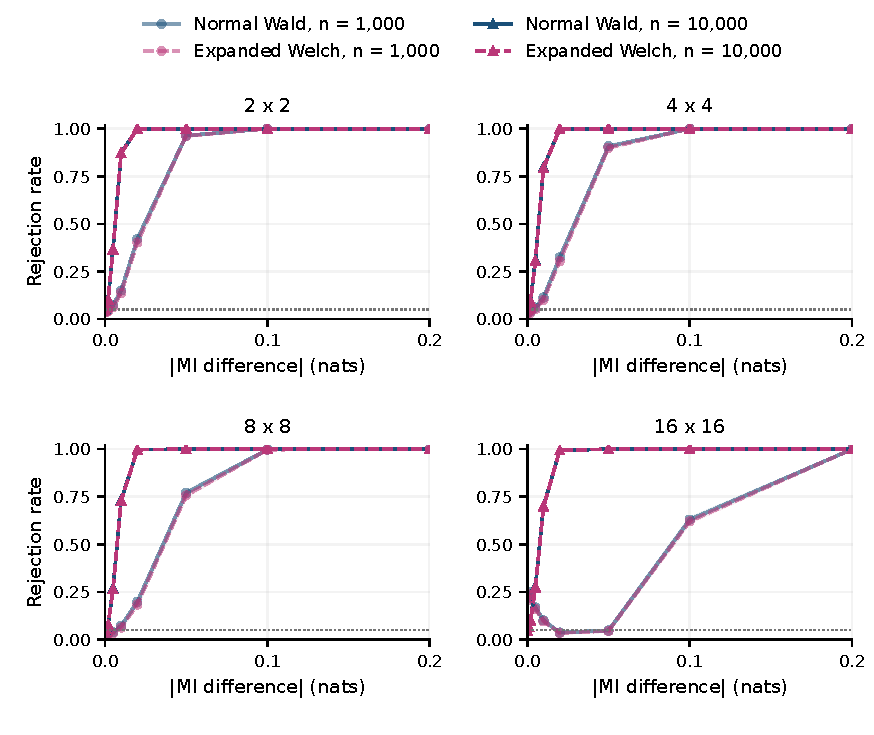
\includegraphics{focused_detection_sizes_full.pdf}
\caption{Full-range rejection rates under different-skew margins.}
\label{fig:focused-detection-full}
\end{figure}

At \(n=1{,}000\), power for a 0.05-nat difference falls with table
size: Wald rates are 0.9642, 0.9079, 0.7699 and 0.0471 from
\(2\times2\) through \(16\times16\). The last curve first falls
from its high null rate, then rises to 0.6297 at 0.1 nats and 0.9997
at 0.2. Unequal bias opposes the small negative true differences there,
as discussed in the main results. At \(n=10{,}000\), both methods
detect every simulated 0.05-nat difference at all four sizes.

Figure~\ref{fig:same-detection-sizes} gives the same-skew comparison
over small MI differences at every table size. Circles indicate
\(n=1{,}000\) and triangles \(n=10{,}000\), as in the main size
comparison.

\begin{figure}[H]
\centering
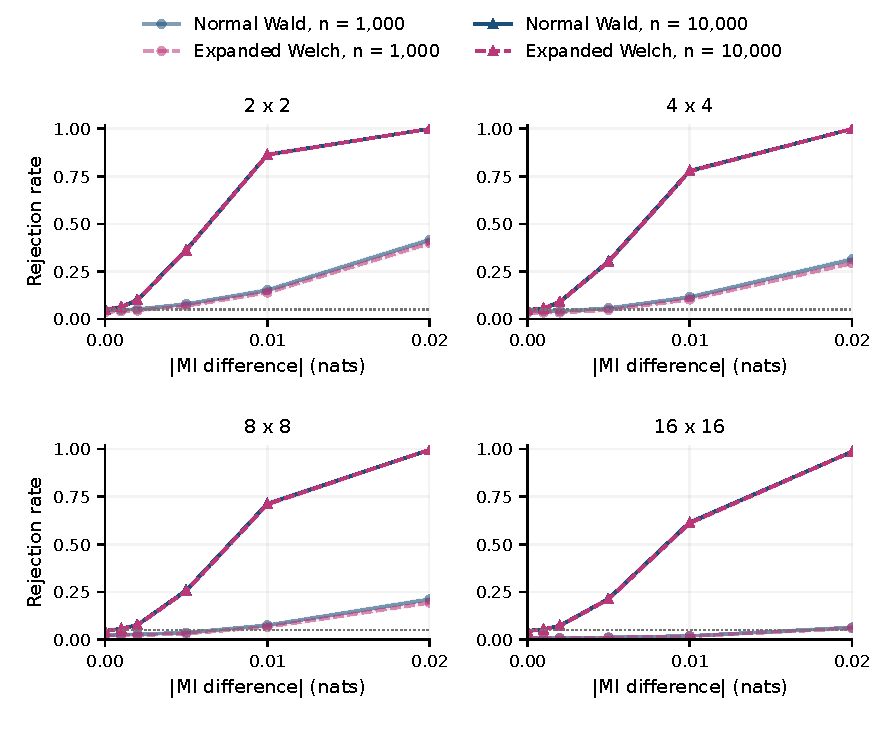
\includegraphics{focused_same_detection_sizes.pdf}
\caption{Rejection rates over small MI differences under same-skew margins.}
\label{fig:same-detection-sizes}
\end{figure}

The same-skew \(16\times16\) comparison has low rather than excessive
null rejection at \(n=1{,}000\), and no comparable initial fall as
the MI difference grows. At 0.01 nats, its difference bias is 0.00092
nats and Wald rejects 370 times, including 14 wrong-direction rejections.
Expanded Welch rejects 339 times, including 12 wrong-direction rejections.
Most rejections have the correct direction, although power remains low.
The alternative populations have different MI, so their biases need not
cancel despite matching margins.

\medskip
\thesisminiheading{Estimated direction among rejections.}

Table~\ref{tab:rejection-direction} examines the \(16\times16\)
different-skew copying populations at two small MI differences.
\(I(P)=0.02\) and \(I(Q)=0.02+|\Delta|\), so the true signed
difference is negative. The table counts rejections with
\(\Deltahat>0\), which incorrectly indicate larger MI for \(P\),
alongside the total number of rejections.

\begin{table}[H]
\centering
\small
\caption{Estimated direction among two-sided rejections.}
\label{tab:rejection-direction}
\begin{tabular}{@{}rrrrrr@{}}
\toprule
& & \multicolumn{2}{c}{Normal Wald} & \multicolumn{2}{c}{Expanded Welch}\\
\cmidrule(lr){3-4}\cmidrule(l){5-6}
\(n\) & \(|\Delta|\) & Rejections & Opposite sign & Rejections & Opposite sign\\
\midrule
1,000 & 0.01 & 2,010 & 2,009 & 1,906 & 1,905\\
1,000 & 0.02 & 725 & 713 & 680 & 669\\
10,000 & 0.01 & 13,984 & 0 & 13,935 & 0\\
10,000 & 0.02 & 19,863 & 0 & 19,862 & 0\\
\bottomrule
\end{tabular}

\end{table}

At \(n=1{,}000\) and a 0.01-nat difference, only one rejection
for each method has the correct estimated direction. At 0.02 nats,
713 of 725 Wald rejections and 669 of 680 Expanded Welch rejections
still have the opposite sign. The larger cutoff reduces rejection
without changing any estimated difference. At \(n=10{,}000\), all
rejections in these comparisons have the correct negative sign,
accompanying the much smaller bias and improved power.

\section{Four-cell construction check}

\thesisminiheading{Representative \(4\times4\) comparison.}

Table~\ref{tab:construction-check} compares the copying and four-cell
populations at matched \(4\times4\) different-skew margins and MI
targets. Constructions use independent repetitions; within each
construction, both tests receive the same table pairs.

\begin{table}[H]
\centering
\small
\caption{Rejection and difference bias under two population constructions.}
\label{tab:construction-check}
\begin{tabular}{@{}lrrrrr@{}}\toprule
Construction & \(n\) & \(|\Delta|\) & Wald & Expanded & Bias\\\midrule
Copying & 1,000 & 0 & 0.0394 & 0.0331 & -0.00012\\
Copying & 1,000 & 0.01 & 0.1132 & 0.1013 & -0.00004\\
Copying & 10,000 & 0 & 0.0481 & 0.0473 & -0.00001\\
Copying & 10,000 & 0.01 & 0.7962 & 0.7940 & 0.00002\\
Four-cell & 1,000 & 0 & 0.0403 & 0.0345 & -0.00018\\
Four-cell & 1,000 & 0.01 & 0.1148 & 0.1032 & -0.00018\\
Four-cell & 10,000 & 0 & 0.0502 & 0.0494 & -0.00001\\
Four-cell & 10,000 & 0.01 & 0.7865 & 0.7844 & -0.00003\\
\bottomrule\end{tabular}

\end{table}

The same qualitative method comparison persists: at \(n=1{,}000\),
Expanded Welch lowers an already-low null rate and reduces power;
at 10,000 its effect is smaller. The construction still changes the
estimated power. For the 0.01-nat difference at \(n=10{,}000\),
Wald's estimated power is 0.7962 under copying and 0.7865 under the four-cell
transfer. The difference, 0.0098, has approximate independent-stream
95\% interval [0.0018, 0.0177].

\medskip
\thesisminiheading{Sparse \(16\times16\) comparison.}

Table~\ref{tab:large-construction-check} tests the larger-table failure
under the same two constructions. Both use different-skew margins
\(m_{16}(0.7)\) for \(P\) and \(m_{16}(0.8)\) for \(Q\), with
the MI targets and sample sizes matched. MCSE denotes the Monte Carlo
standard error of the difference bias. Opposite W/E reports the percentage of Wald and Expanded Welch
rejections whose estimated difference has the opposite sign to the
population difference. It applies only to the nonzero alternative.

\begin{table}[H]
\centering
\small
\caption{Matched \(16\times16\) comparisons under two constructions.}
\label{tab:large-construction-check}
\setlength{\tabcolsep}{4.5pt}
\begin{tabular}{@{}rlrrr@{}}
\toprule
\(n\) & Construction & Normal Wald & Expanded Welch & Valid W/E (\%)\\
\midrule
\multicolumn{5}{@{}l}{\(I(P)=I(Q)=0.02\): false positives}\\
1,000 & Copying & 0.2522 [0.2462, 0.2583] & 0.2402 [0.2343, 0.2462] & 100.0/100.0\\
1,000 & Four-cell & 0.3095 [0.3031, 0.3159] & 0.2977 [0.2914, 0.3041] & 100.0/100.0\\
10,000 & Copying & 0.0463 [0.0434, 0.0492] & 0.0453 [0.0425, 0.0482] & 100.0/100.0\\
10,000 & Four-cell & 0.0499 [0.0470, 0.0530] & 0.0491 [0.0462, 0.0522] & 100.0/100.0\\
\midrule
\multicolumn{5}{@{}l}{\(I(P)=0.02,\ I(Q)=0.03\): power}\\
1,000 & Copying & 0.1005 [0.0964, 0.1047] & 0.0953 [0.0913, 0.0994] & 100.0/100.0\\
1,000 & Four-cell & 0.1247 [0.1202, 0.1294] & 0.1176 [0.1132, 0.1221] & 100.0/100.0\\
10,000 & Copying & 0.6992 [0.6928, 0.7055] & 0.6968 [0.6903, 0.7031] & 100.0/100.0\\
10,000 & Four-cell & 0.6323 [0.6256, 0.6390] & 0.6297 [0.6229, 0.6363] & 100.0/100.0\\
\bottomrule
\end{tabular}
\par\medskip
\begin{tabular}{@{}rlrrrrr@{}}
\toprule
\(n\) & Construction & Bias & MCSE & Obs. SD & Est./obs. & Opposite W/E (\%)\\
\midrule
\multicolumn{7}{@{}l}{\(I(P)=I(Q)=0.02\)}\\
1,000 & Copying & +0.02960 & 0.00010 & 0.01449 & 1.94 & ---\\
1,000 & Four-cell & +0.03145 & 0.00011 & 0.01568 & 1.67 & ---\\
10,000 & Copying & -0.00088 & 0.00003 & 0.00387 & 1.07 & ---\\
10,000 & Four-cell & -0.00097 & 0.00003 & 0.00426 & 1.05 & ---\\
\midrule
\multicolumn{7}{@{}l}{\(I(P)=0.02,\ I(Q)=0.03\)}\\
1,000 & Copying & +0.03061 & 0.00011 & 0.01564 & 1.81 & 99.95/99.95\\
1,000 & Four-cell & +0.03136 & 0.00012 & 0.01671 & 1.60 & 99.96/99.96\\
10,000 & Copying & -0.00094 & 0.00003 & 0.00433 & 1.05 & 0.00/0.00\\
10,000 & Four-cell & -0.00092 & 0.00003 & 0.00468 & 1.04 & 0.00/0.00\\
\bottomrule
\end{tabular}

\end{table}

At \(n=1{,}000\), the four-cell null has difference bias
0.03145 nats and false-positive rates 0.3095 for Wald and 0.2977 for
Expanded Welch. Both rates exceed those under copying, where the
corresponding bias is 0.02960 nats. For the 0.01-nat alternative,
the four-cell bias of 0.03136 moves the mean estimated difference to
approximately \(-0.01+0.03136=0.02136\) nats. This is positive
although \(Q\) has larger population MI. Opposite-sign counts are
2,493 of 2,494 Wald rejections and 2,350 of 2,351 Expanded Welch
rejections; only one rejection for each method has the correct sign.
The sparse-table bias and reversed estimated ordering therefore persist
under both tested constructions.

At \(n=10{,}000\), the four-cell null rates are 0.0499 and 0.0491,
with much smaller difference bias. Every rejection at the alternative
has the correct estimated direction under either construction.
Power nevertheless differs: Wald gives 0.6992 under copying and
0.6323 under the four-cell transfer. The MI difference biases under
copying and the four-cell transfer are similar, but the
observed SD rises from approximately 0.00433 to 0.00468 nats, making
the same population difference harder to detect under the transfer.

\medskip
\thesisminiheading{Matched same-skew comparisons.}

Table~\ref{tab:same-construction-check} repeats the construction check
with \(m_k(0.8)\) margins in both populations, keeping MI targets and
sample sizes matched between constructions.

\begin{table}[H]
\centering
\small
\setlength{\tabcolsep}{4pt}
\caption{Same-skew comparisons under copying and four-cell constructions.}
\label{tab:same-construction-check}
\begin{tabular}{@{}rrlrrrrr@{}}\toprule
Size & \(n\) & Construction & \(|\Delta|\) & Wald & Expanded & Bias & DF\\\midrule
\(4\times4\) & 1,000 & Copying & 0 & 0.0392 & 0.0319 & -0.00006 & 33.45\\
\(4\times4\) & 1,000 & Four-cell & 0 & 0.0385 & 0.0315 & -0.00001 & 33.69\\
\(4\times4\) & 1,000 & Copying & 0.01 & 0.1152 & 0.1033 & -0.00002 & 40.22\\
\(4\times4\) & 1,000 & Four-cell & 0.01 & 0.1178 & 0.1059 & -0.00005 & 41.28\\
\(4\times4\) & 10,000 & Copying & 0 & 0.0481 & 0.0472 & -0.00003 & 279.00\\
\(4\times4\) & 10,000 & Four-cell & 0 & 0.0490 & 0.0481 & +0.00001 & 275.62\\
\(4\times4\) & 10,000 & Copying & 0.01 & 0.7790 & 0.7768 & +0.00004 & 343.87\\
\(4\times4\) & 10,000 & Four-cell & 0.01 & 0.7665 & 0.7642 & -0.00001 & 349.26\\
\(16\times16\) & 1,000 & Copying & 0 & 0.0065 & 0.0059 & +0.00004 & 78.89\\
\(16\times16\) & 1,000 & Four-cell & 0 & 0.0107 & 0.0095 & -0.00011 & 81.17\\
\(16\times16\) & 1,000 & Copying & 0.01 & 0.0185 & 0.0170 & +0.00092 & 84.00\\
\(16\times16\) & 1,000 & Four-cell & 0.01 & 0.0292 & 0.0266 & -0.00007 & 92.27\\
\(16\times16\) & 10,000 & Copying & 0 & 0.0450 & 0.0440 & +0.00002 & 265.71\\
\(16\times16\) & 10,000 & Four-cell & 0 & 0.0465 & 0.0456 & 0.00000 & 270.31\\
\(16\times16\) & 10,000 & Copying & 0.01 & 0.6146 & 0.6113 & -0.00005 & 307.66\\
\(16\times16\) & 10,000 & Four-cell & 0.01 & 0.5464 & 0.5433 & -0.00001 & 348.92\\
\bottomrule\end{tabular}

\end{table}

At \(16\times16\) and \(n=1{,}000\), the same-skew Wald null
rates are 0.0065 under copying and 0.0107 under the four-cell transfer,
rather than the excessive different-skew rates. The null difference
biases are close to zero because the population tables and sample sizes
match within each construction. At the alternative, the four-cell
construction gives Wald power 0.0292, compared with 0.0185 under copying;
both remain low. The median degrees of freedom are 92.27 and 84.00,
respectively, but mean squared standard error still exceeds observed
variance, with ratios 1.56 and 1.82.

At \(n=10{,}000\), same-skew null rates are closer to 0.05 under
both constructions. At the \(16\times16\) alternative, Wald power
is 0.6146 under copying and 0.5464 under the four-cell transfer. The
median degrees of freedom are now above 300 in both cases, and Expanded
Welch changes those rates only slightly. Its larger rejection cutoff
does not explain the substantial power difference between constructions.

\section{Unequal sample sizes at a fixed total}
\label{sec:allocation-check}

Table~\ref{tab:allocation-check} compares three allocations of 2,000
observations between the same copying \(4\times4\) populations.
The row and column margins are \((0.7,0.1,0.1,0.1)\) in \(P\) and
\((0.8,0.2/3,0.2/3,0.2/3)\) in \(Q\). Both MI values are 0.02 nats
under the null; under the alternative, \(I(Q)=0.03\) and
\(\Delta=-0.01\) nats. Balanced results are reused from the main study.
Different allocations use independent repetitions, whereas
the two methods receive the same samples within each allocation.

Valid W/E gives the valid-result percentages for the two methods.

\begin{table}[H]
\centering
\small
\caption{Rejection and estimation diagnostics at fixed total sample size.}
\label{tab:allocation-check}
\begin{tabular}{@{}lrrr@{}}
\toprule
\((n_P,n_Q)\) & Normal Wald & Expanded Welch & Valid W/E (\%)\\
\midrule
\multicolumn{4}{@{}l}{\(I(P)=I(Q)=0.02\): false positives}\\
\((1000,1000)\) & 0.0394 [0.0368, 0.0422] & 0.0331 [0.0307, 0.0357] & 100.0/100.0\\
\((400,1600)\) & 0.0463 [0.0435, 0.0493] & 0.0306 [0.0283, 0.0331] & 100.0/100.0\\
\((1600,400)\) & 0.0454 [0.0426, 0.0484] & 0.0252 [0.0231, 0.0274] & 100.0/100.0\\
\midrule
\multicolumn{4}{@{}l}{\(I(P)=0.02,\ I(Q)=0.03\): power}\\
\((1000,1000)\) & 0.1132 [0.1089, 0.1177] & 0.1013 [0.0972, 0.1056] & 100.0/100.0\\
\((400,1600)\) & 0.1295 [0.1249, 0.1342] & 0.0997 [0.0956, 0.1039] & 100.0/100.0\\
\((1600,400)\) & 0.0540 [0.0509, 0.0572] & 0.0340 [0.0316, 0.0366] & 100.0/100.0\\
\bottomrule
\end{tabular}
\par\medskip
\begin{tabular}{@{}lrrrr@{}}
\toprule
\((n_P,n_Q)\) & Difference bias & Observed SD & Est./obs. & Median DF\\
\midrule
\multicolumn{5}{@{}l}{\(I(P)=I(Q)=0.02\)}\\
\((1000,1000)\) & -0.00012 & 0.01053 & 1.06 & 35.70\\
\((400,1600)\) & +0.00068 & 0.01374 & 1.10 & 14.42\\
\((1600,400)\) & -0.00144 & 0.01376 & 1.11 & 10.97\\
\midrule
\multicolumn{5}{@{}l}{\(I(P)=0.02,\ I(Q)=0.03\)}\\
\((1000,1000)\) & -0.00004 & 0.01167 & 1.07 & 42.10\\
\((400,1600)\) & +0.00073 & 0.01431 & 1.10 & 16.95\\
\((1600,400)\) & -0.00143 & 0.01610 & 1.08 & 13.48\\
\bottomrule
\end{tabular}

\end{table}

With equal MI, Wald rejects at 0.0394 for balanced samples, 0.0463 at
\((n_P,n_Q)=(400,1600)\), and 0.0454 at \((1600,400)\). Expanded Welch lowers these
rates to 0.0331, 0.0306 and 0.0252, respectively. The imbalance therefore
does not create excessive Wald rejection in these settings, and the
larger Expanded Welch cutoff makes already-low rates lower. The null median
degrees of freedom fall from 35.70 under balance to 14.42 and 10.97, increasing the
cutoff from the Student \(t\) distribution.

For the 0.01-nat difference, giving \(Q\) only 400 observations lowers
power for both methods. The observed SD rises from 0.01167 nats
under balance to 0.01610; with \(P\) limited to 400, it is 0.01431.
Reversing the allocation also changes the remaining difference bias:
\(+0.00073\) nats when \(P\) has fewer observations and
\(-0.00143\) when \(Q\) has fewer. The null biases have the same
signs, with Monte Carlo standard error about 0.00010 in either case.
Mean squared standard error exceeds observed variance in each comparison.

Table~\ref{tab:same-allocation-check} repeats the allocations under same
skew. Both populations use
\((0.8,0.2/3,0.2/3,0.2/3)\) margins. They are identical under the null,
but differ in MI under the alternative. The balanced rows reuse the
main-study samples.

\begin{table}[H]
\centering
\small
\setlength{\tabcolsep}{4pt}
\caption{Same-skew allocation comparisons at a fixed total of 2,000 observations.}
\label{tab:same-allocation-check}
\begin{tabular}{@{}rrrrrrrr@{}}\toprule
\(n_P\) & \(n_Q\) & \(|\Delta|\) & Wald & Expanded & Bias & Est./obs. & DF\\\midrule
400 & 1,600 & 0 & 0.0458 & 0.0265 & +0.00128 & 1.114 & 11.27\\
1,000 & 1,000 & 0 & 0.0392 & 0.0319 & -0.00006 & 1.065 & 33.45\\
1,600 & 400 & 0 & 0.0423 & 0.0234 & -0.00148 & 1.112 & 11.33\\
400 & 1,600 & 0.01 & 0.1300 & 0.0946 & +0.00129 & 1.081 & 13.38\\
1,000 & 1,000 & 0.01 & 0.1152 & 0.1033 & -0.00002 & 1.043 & 40.22\\
1,600 & 400 & 0.01 & 0.0506 & 0.0340 & -0.00124 & 1.077 & 13.70\\
\bottomrule\end{tabular}

\end{table}

With identical null populations, unequal allocation still produces
residual biases of opposite signs: approximately 0.00128 nats when
\(P\) has 400 observations and \(-0.00148\) when \(Q\) has 400.
The leading analytic corrections have already been applied, so these
values show the remaining sample-size dependence of the MI bias.
Median degrees of freedom fall from 33.45 under balance to approximately
11.3 under either imbalance, and Expanded Welch reduces the null rates
from 0.0458 and 0.0423 to 0.0265 and 0.0234.

Under the alternative, allocating more observations to \(Q\) gives Wald
power 0.1300, compared with 0.1152 under balance; allocating fewer to
\(Q\) gives 0.0506. Expanded Welch instead gives 0.0946, 0.1033 and
0.0340 for those allocations. Its median degrees of freedom drop from
40.22 under balance to about 13--14 under imbalance.

\section{Holm adjustment for the application}
\label{sec:application-holm}

Table~\ref{tab:application-holm} gives the raw and adjusted p-values for
all six comparisons used to select the online-shopping application.
Each tests equal predictor--outcome MI between two groups. Adult compares
female and male records using education (16 categories) or occupation
(14 categories) and income above US\$50,000 \citep{becker1996}. Its
training and test partitions are combined without survey weights;
records with missing occupation are excluded only from that comparison.
Student Performance compares schools GP and MS using Portuguese-language
course records, study time (four levels) or maternal education (five levels),
and a final grade of at least 10 \citep{cortez2008}. The shopping
comparisons use month or weekend and purchasing among new and returning visitors.

\begin{table}[H]
\centering
\small
\caption{Raw and Holm-adjusted p-values for the six exploratory comparisons.}
\label{tab:application-holm}
\setlength{\tabcolsep}{4pt}
\begin{tabularx}{\textwidth}{@{}>{\raggedright\arraybackslash}Xrrrr@{}}
\toprule
& \multicolumn{2}{c}{Normal Wald} & \multicolumn{2}{c}{Expanded Welch}\\
\cmidrule(lr){2-3}\cmidrule(l){4-5}
Comparison & Raw & Adjusted & Raw & Adjusted\\
\midrule
Adult: occupation & \(1.18\times10^{-44}\) & \(7.10\times10^{-44}\) & \(1.64\times10^{-42}\) & \(9.81\times10^{-42}\)\\
Adult: education & \(1.89\times10^{-34}\) & \(9.45\times10^{-34}\) & \(4.93\times10^{-33}\) & \(2.46\times10^{-32}\)\\
Online Shoppers: month & \(4.71\times10^{-5}\) & \(1.89\times10^{-4}\) & \(3.73\times10^{-4}\) & \(1.49\times10^{-3}\)\\
Student Performance: study time & 0.1982 & 0.5946 & 0.2339 & 0.7016\\
Student Performance: maternal education & 0.8361 & 1 & 0.8468 & 1\\
Online Shoppers: weekend & 0.9554 & 1 & 0.9601 & 1\\
\bottomrule
\end{tabularx}
\end{table}

Holm's multiple-testing adjustment is applied separately to each method's
six p-values \citep{holm1979}. Order the raw p-values from smallest to largest and
multiply them by 6, 5, 4, 3, 2 and 1, respectively. Moving through that
order, replace any value smaller than the preceding adjusted value by
that preceding value, and cap the results at one. The month--purchase comparison has the
third-smallest raw p-value for both methods, and the earlier adjusted
values are smaller, so its adjusted p-value is four times its raw value.
Both adjusted month p-values remain below 0.05.
